\section{Classification Evaluation}\label{ClassificationEvaluation} % start a new section and label it for cross-referencing

\subsection{Performance evaluation}

Performance evaluation in classification is based on \emph{accuracy} and \emph{error rate}.

Consider a typical classification problem:
\begin{equation}
    f: X \xrightarrow{} Y \\
\end{equation}
$\mathcal{D}$: probability distribution over X \\
$\mathcal{S}$: sample of n instances drawn from X \\
Consider a hypothesis h, solution of a learning algorithm obtained from S. What is the best estimate of the accuracy of h over future instances drawn from the same distribution? What is the probable error in this accuracy estimate?

\subsubsection{true error and sample error}
    true error of hypothesis h with respect to target function f and distribution D is the probability that h will misclassify an instance drawn at random according to D
\begin{equation}
    error_{\mathcal{D}}(h) \equiv \prod_{x \in D} [\sigma (f(x) \neq h(x))]
\end{equation}
The sample error of h with respect to target function f and data sample
S is the proportion of examples h misclassifies
\begin{equation}
    error_{\mathcal{S}}(h) \equiv \frac{1}{n}\sum_{x \in S} \sigma (f(x) \neq h(x))
\end{equation}
where $\sigma (f(x) \neq h(x))$ is equal to 1 if $f(x) \neq h(x)$ and 0 otherwise.

Note: $accuracy(h) = 1 - error(h)$

The true error cannot be computed, the sample error is computed only
on a small data sample.

If $accuracyS (h)$ is very high, but $accuracyD(h)$ is poor, then our system
would not be very useful.

\subsubsection{Estimating Bias}

\begin{equation}
    bias = E[error_S (h)] - error_D (h)
\end{equation}

\subsubsection{Confidence interval}
with approximate N\% probabiliry, $error:D (h)$ lies in interval
\begin{equation}
    error_S (h) +- z_{N} \sqrt{\frac{error_S(h) (1-error_S(h))}{n}}
\end{equation}
where
\begin{figure}[H]
    \centering
    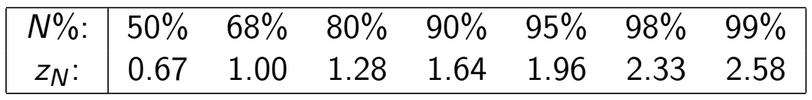
\includegraphics[width=12cm,keepaspectratio]{images/Classification Evaluation/Screenshot_20221004_125528.png}
    \caption{Value of z$_{N}$  based on the $N\%$ chosen}
    \label{fig:z_N}
\end{figure}

\subsubsection{K-Fold Cross Validation}

Partition data set D into k disjoint sets $S_1, S_2, . . . , S_k (|S_i| > 30)$ and then use one set as test set while the remaining sets as training set

The error is
\begin{equation}
    error_{L,D} \equiv \frac{1}{k}\sum_{i = 1}^{k}\sigma_i
\end{equation}

note: $accuracy_{L,D} = 1 - error_{L, D}$

\subsubsection{Comparing learning algorithms}

If we have two hypothesis $h_1, h_2$, the true comparison is
\begin{equation}
    d \equiv error_D (h_1) - error_D (h_2)
\end{equation}

and its estimator is

\begin{equation}
    \hat{d} \equiv error_{S_1} (h_1) - error_{S_2} (h_2)
\end{equation}

$\hat{d}$ is an unbiased estimator for d, iff $h_1, h_2, S_1 and S_2$ are independent from each other
\begin{equation}
    E[\hat{d}] = d
\end{equation}

to estimate which algorithm is better we would like to estimate:
\begin{equation}
    E_{S\subset D}[error_D (L_A(S)) - error_D(L_B(S))]
\end{equation}

where L(S) is the hypothesis output by learner L using training set S

this measure can be approximated by K-Fold cross validation

\subsection{Performance Metrics}

\begin{figure}[H]
    \centering
    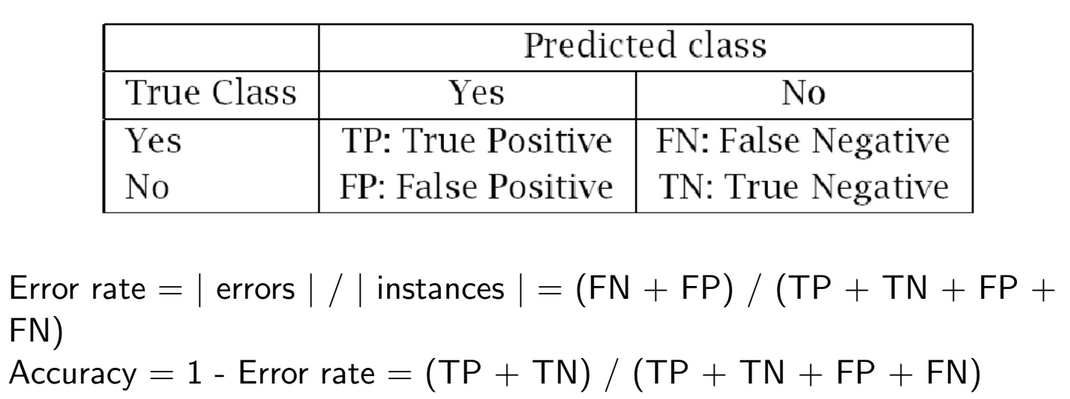
\includegraphics[width=12cm,keepaspectratio]{images/Classification Evaluation/Screenshot_20221004_131728.png}
    \caption{}
    \label{fig:image2}
\end{figure}

Sometimes accuracy is not enough. Imagine a dataset of 90 cats and 10 dogs. An algorithm that always returns "cat" will have 90$\%$ accuracy while a classification algorithm may have 85$\%$, but actually be good.

Unbalanced data sets are very common in problems related to anomaly detection.

Other Performance metrics are:

\begin{figure}[H]
    \centering
    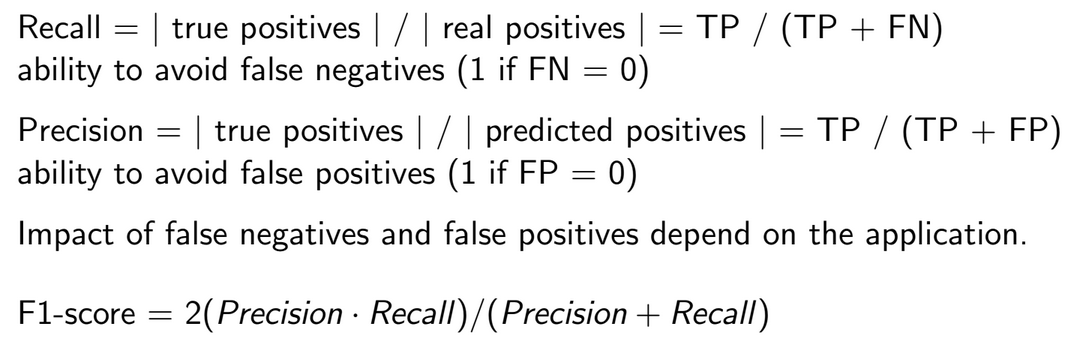
\includegraphics[width=12cm,keepaspectratio]{images/Classification Evaluation/Screenshot_20221004_134809.png}
    \caption{}
    \label{fig:image_metric_1}
\end{figure}

\begin{figure}[H]
    \centering
    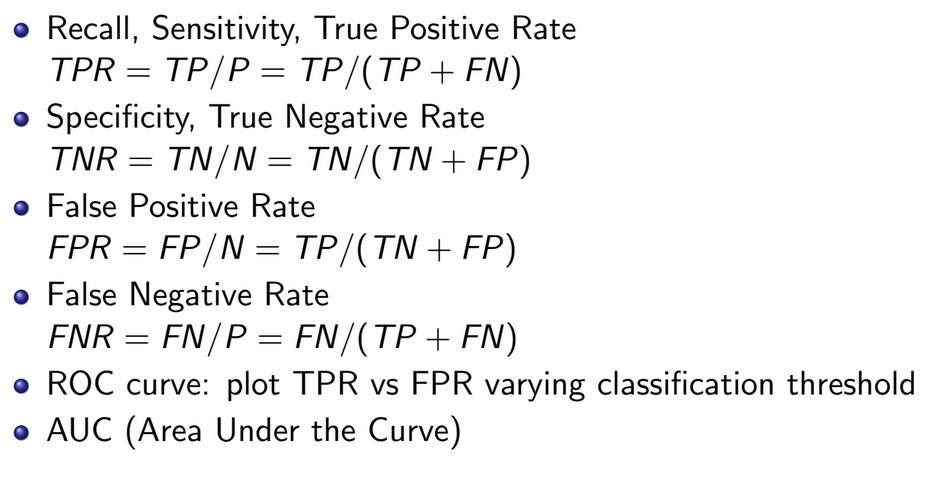
\includegraphics[width=12cm,keepaspectratio]{images/Classification Evaluation/Screenshot_20221004_135110.png}
    \caption{}
    \label{fig:image_metric_2}
\end{figure}